\chapter{Verification}

\section{Introduction}

Even though the controller designs enabled the \gls{twip} system to remain upright, no analysis was performed to determine how stable the system is. All previous work exploited some aspects of the system's dynamics in order to improve response; the approaches themselves failed to yield guarantees of the system's overall stability. Accordingly, the next step required is formally verifying whether the \gls{twip} meets a desired specification. Digital systems have a long history with formal verification techniques---their binary nature lends themselves well to closing a chain of evidence between possible inputs and desired system behavior. \\

Dynamical, and also analog, systems have numerous complications when comparing response behavior to a specification. Firstly, the continuous time domain restricts all possible inputs from being explored in finite time. Secondly, high variability can exist in the components, making it difficult to verify a system without extensive measurements. Lastly, the models used in the verification process have inaccuracies, so uncertainty can originate from the model itself. There exists an implicit assumption that the system model is sufficiently accurate in the validation of its controllers. This assumption invites additional verification via inverse modeling post-build: the model's behavior and actual behavior should be compared. \\

How is a dynamical system like an inverted pendulum verified? A collection of inputs can be simulated and then checked so that the IP is expected to converge to a stable value. In many cases, however, the use of single trajectories can lead to misleading results. Instead, the system's state space can be explored in order to determine specification adherence. In general, allow a system to exist in generalized coordinates $\bm{x}$ with the time derivative $\dot{\bm{x}}$ and input variables $\bm{u}(t)$. There exists a function, $\bm{f}$, then,

\begin{equation}
    \bm{f} \left( \bm{x}(t), \dot{\bm{x}}(t), \bm{u}(t) \right) = \bm{0}.
\end{equation}

In $\bm{x}(t)$, there are state variables, $\bm{x}^z$ that spans the state space of the system. Further, an output function should also be specified. In the case of an ODE system, this may be one or a combination of the state variables; in DAE representation, this can be any algebraic expression involving the state variables. This measure---a dynamical system's state space---requires additional transformations because the state space for a system is not unique. In verification, the common approach is to reduce the model into a \textit{canonical form} that yields one unique representation for every system. In state space verification, several canonical forms can be used, one of the more common ones being Kronecker canonical form due to its relative ease of computation \cite{marz1992numerical}. \\

Often a collection of values in the state space are attributed to a logical state. In the case of the TWIP, when the robot's tilt angle and tilt angular rate are nearly zero, the robot can be considered \textit{stabilized}. Otherwise the robot can either be \textit{stabilizing} or \textit{unstable}---the difference being that one is able to transition to a \textit{stabilized} state while the other not. The margins between \textit{stabilized} and \textit{stabilizing} are arbitrary, specified by the behavioral description. Of course, the controller design attempts to minimize both the \textit{stabilized} and \textit{unstable} regions, while maximizing the \textit{stabilizing} region. Importantly, it would unreasonable to expect arbitrary convergence time, and so the state transitions must occur within a desired time interval. Good controller designs are able to converge quickly while still possessing the acceptable region sizes mentioned.   

\subsection{First Order Example}
Three controlled first order systems are designed to converge on the control point, $x_c = 3$:

\begin{enumerate}
    \item $\dot{x} = 3-x$
    \item $\dot{x} = x \left( 1 - \frac{x}{3} \right)$
    \item $\dot{x} = - \ln\left( \frac{x}{3} \right)$
\end{enumerate}

Some steady state error is permitted, so the region $2.5 < x(t) < 3.5$ is permitted to the target region. Valid starting states for the system is $x_0 \in [2, 4]$. \\

Solving for the ODE's directly yields the solutions. Figure \ref{fig:fregions} shows the differential equation plots. Table \ref{tab:fregions} shows that systems 1 and 2 pass verification, while system 3 does not. This method, observing, how the initial conditions change the closed form solution, is not a viable solution when the state space is highly dimensional. Numerical techniques, like solving the ODE backwards in time, can find these cases without requiring a symbolic solution. 

\begin{figure}

\centering
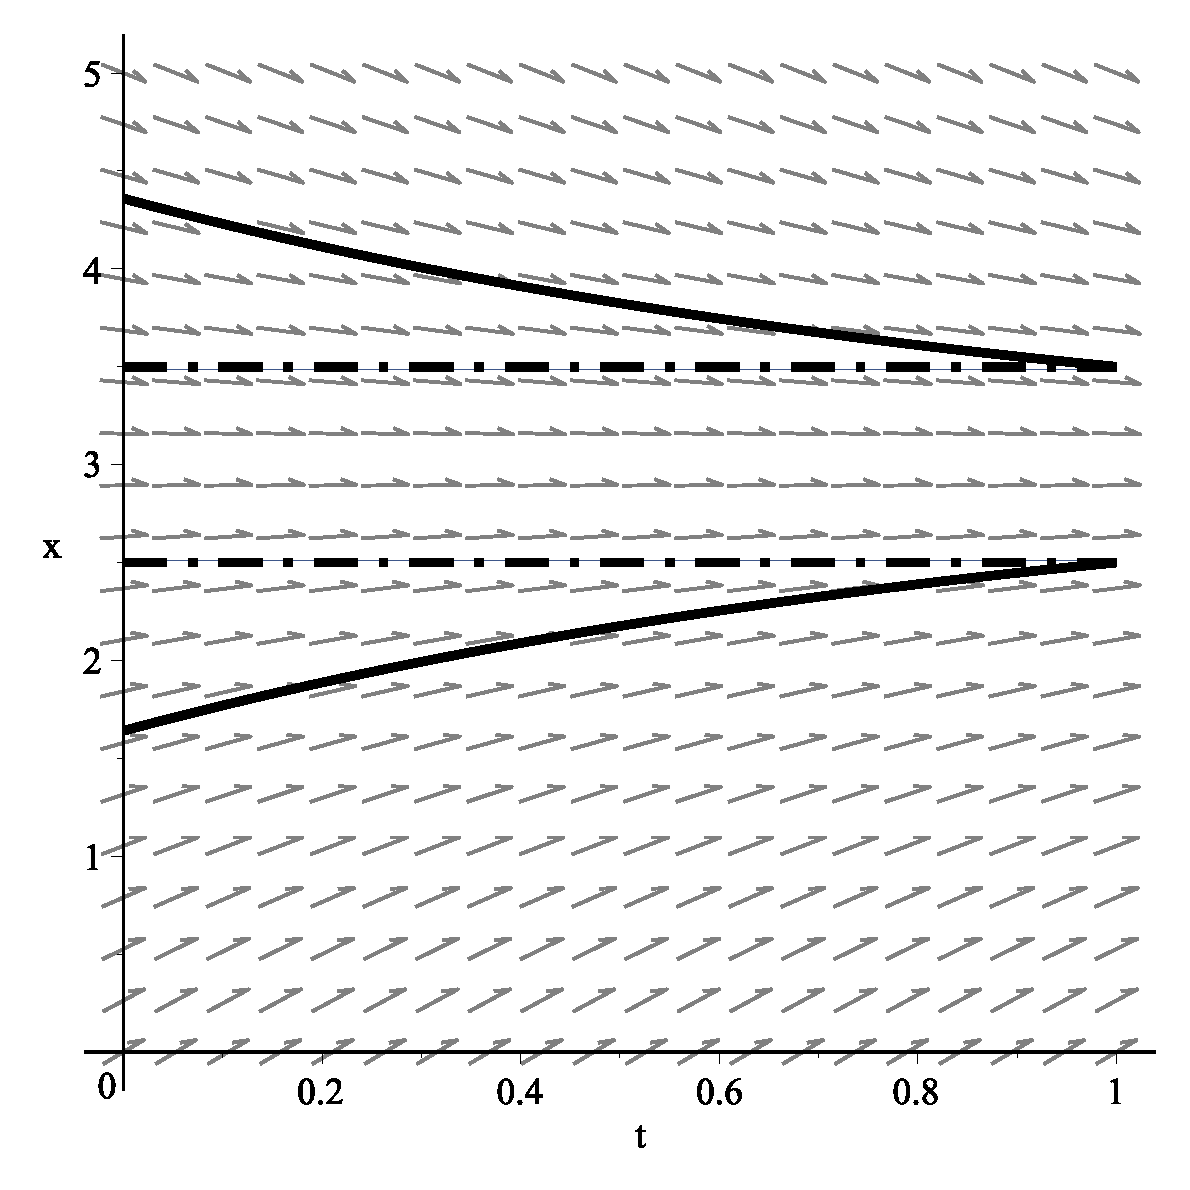
\includegraphics[width=.3\textwidth]{img/p1_regions.eps}\hfill
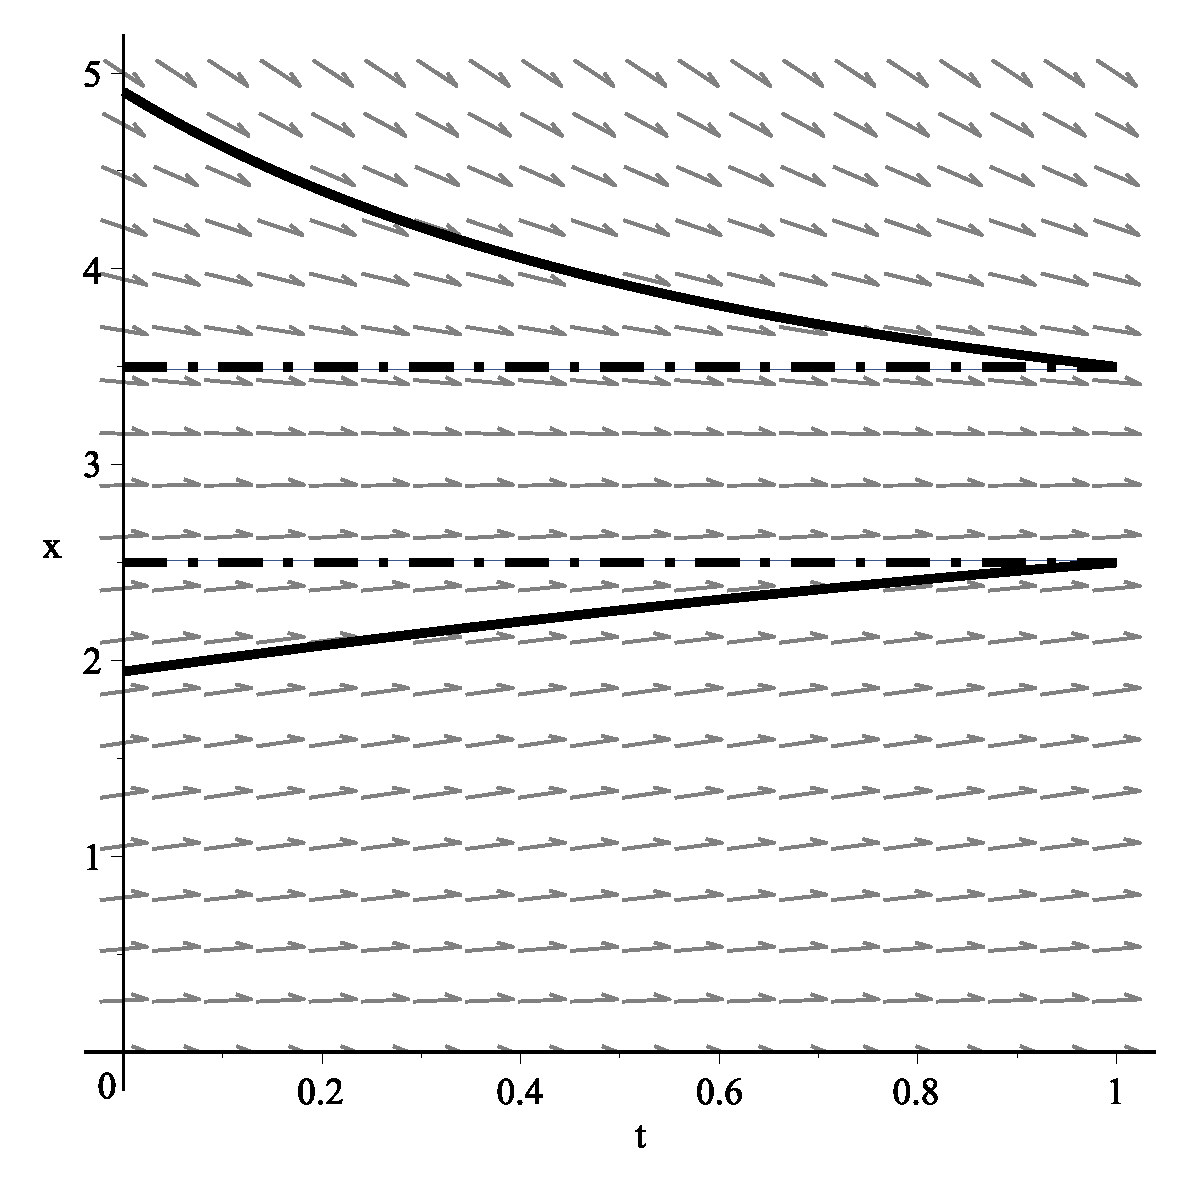
\includegraphics[width=.3\textwidth]{img/p2_regions.eps}\hfill
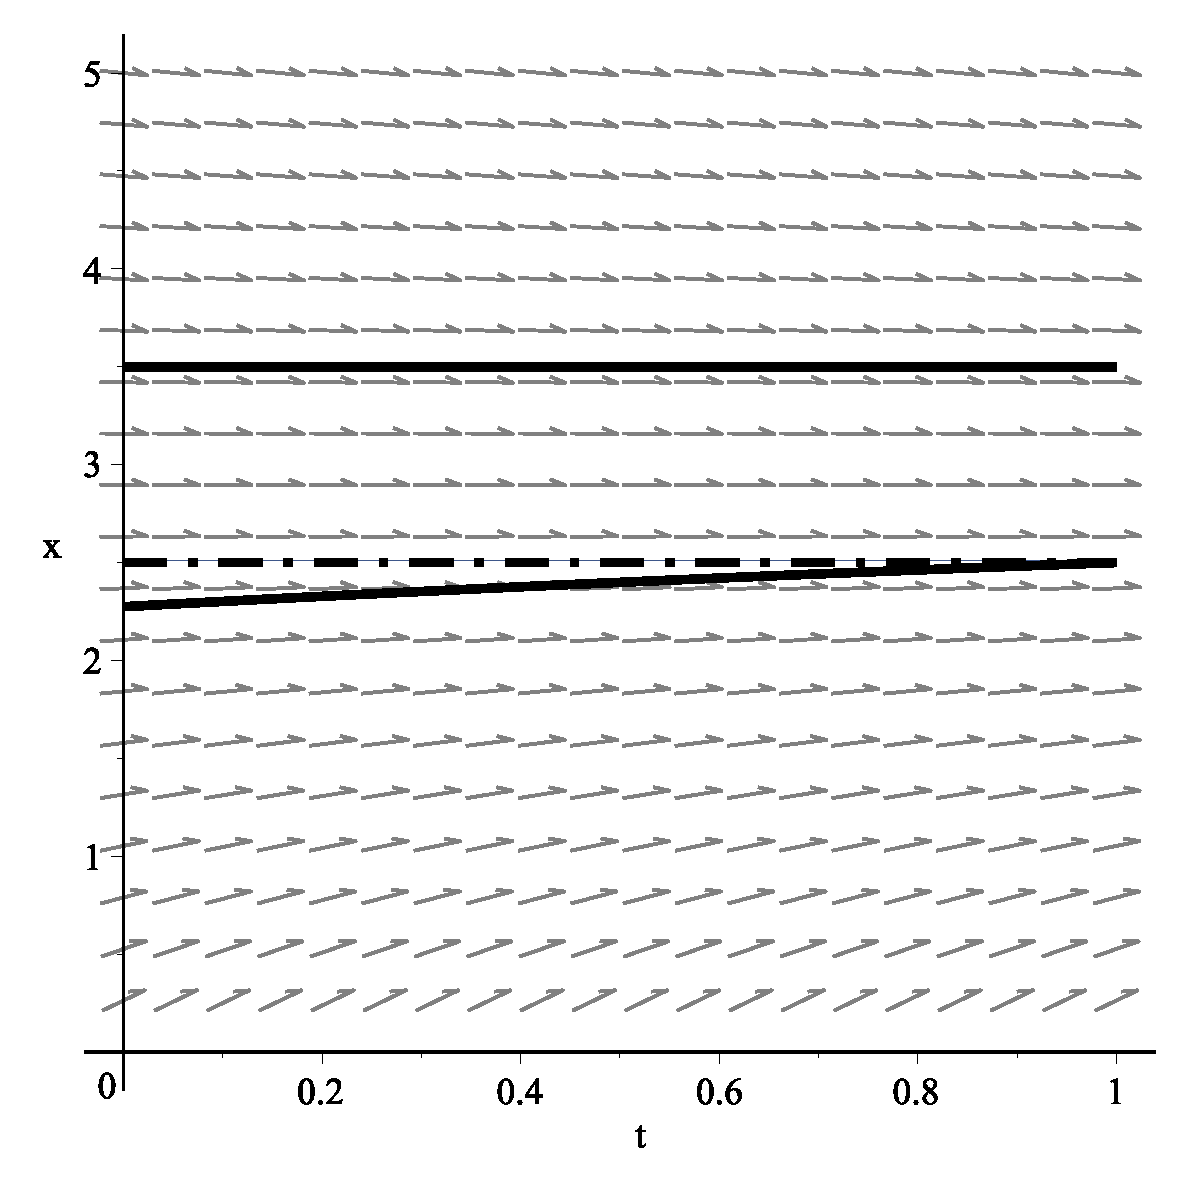
\includegraphics[width=.3\textwidth]{img/p3_regions.eps}

\caption{Presented are the differential equation plots of the first order differential systems being verified. The region enclosed by the solid line indicate solutions $x(t)$ that exhibit to the desired behavior. Even though all systems will converge to the desired setpoint, functions outside of the region will not do it in the specified time interval $t=1$.   }
\label{fig:fregions}
\end{figure}

\begin{table}[h]
    \centering
    \begin{tabular}{c||c||c|c|c}
    & Specification & System 1 & System 2 & System 3  \\ \hline \hline
    Min $x_0$ &  <2 &  \textbf{1.64} & \textbf{1.94} & 2.27 \\ \hline
    Max $x_0$ & >4 &  \textbf{4.36} & \textbf{4.90} & 2.50 \\ \hline 
    \end{tabular}
    \caption{The system regions are checked against the desired specification.As the goal was fairly attainable, systems 1 and 2 pass verification with considerable margins. Note that system 3 has a region that does not converge to the setpoint when $x_0 > 3.5$, making it a poor choice for the design. }
    \label{tab:fregions}
\end{table}

\subsection{\gls{pd} Control for an Inverted Pendulum Example}

Using a simple pendulum model, it is desired to produce a controller that stabilizes an inverted pendulum. The gravitational acceleration present is $g=9.81$ m/s$^2$ and the length is $l=1$ m. The system is considered to be stabilized if it falls within $|\theta - \pi| < \frac{\pi}{16}$ for time $t_c < 2.0$ of the setpoint is considered stable. Using the simplest model,

\begin{equation}
    \bm{f}\left( {\bm{\theta} ,\dot{\bm{\theta}} } \right) = \left[ {\begin{array}{*{20}{c}}
  {{{\dot \theta }_1} - {\theta _2}} \\ 
  {{{\dot \theta }_2} + \frac{g}{l}\sin \left( {{\theta _1}} \right)} + b \theta_2
\end{array}} \right]
\end{equation}

It is clear, then, that the goal is to find initial conditions that converge near the value $\theta = \pi$ as $t \rightarrow \infty $. The control opportunity present is to apply torque to the pendulum. Accordingly, the controlled system is set to a forcing function value,

\begin{equation}
    \ddot \theta (t) + \frac{g}{l}\sin \left( {\theta (t)} \right)  + b \theta_2 = c(t),
\end{equation}

where the input $c(t)$ comes from a controller. In order for the controller to successfully set the system to a desired setpoint, it is necessary for it to have some way of quantifying how close the system if from its desired state. This can be done with an error signal defined as the difference of a system parameter from its setpoint value, $e(t)=\theta_s - \theta(t)$.  For a \gls{pd} controller, this error function's derivative is used to affect the system damping, improving the system's ability to converge to its setpoint. The controlled system becomes


\begin{equation}
    \bm{f_c}\left( {\bm{\theta} ,\dot{\bm{\theta}} } \right) = \left[ {\begin{array}{*{20}{c}}
  {{{\dot \theta }_1} - {\theta _2}} \\ 
  {{{\dot \theta }_2} + \frac{g}{l}\sin \left( {{\theta _1}} \right) + b \theta_2 + {K_D}{\theta _2} - {K_P}\left( {{\theta _s} - {\theta _1}} \right)} 
\end{array}} \right]
\end{equation}

\section{Stability Analysis Overview}

It is known, intuitively, that the robot is stable in certain regions of state space and unstable in others. Determining the \textit{local stability} about equilibria requires formalizing methods of stability analysis. Developing algorithms to determine the \textit{regions of attraction} generally requires algorithms that scale poorly, requiring substantial computational capability. \\

Lyapunov's theory serves as the basis for stability analyses. It is akin to the potential function utilized in physics to determine dynamical behavior. Let $D$ be a compact subset of the state space, containing equilibrium point $\bm{x}_0$ and there exists a function $V:D \rightarrow \bR$. 

\begin{thm}
\textbf{Lyapunov Stability Theorem.} The equilibrium point  $\bm{x}_0$ is stable if $V$ satisfies the following conditions

\begin{enumerate}
    \item $V(\bm{x}) \ge 0$ $\forall \bm{x} \in D$.
    \item $V(\bm{x}) =0$ if and only if $\bm{x} = \bm{x}_0$.
    \item For all $\bm{x}(t) \in D$,
    \begin{equation}
        \dot{V}(\bm{x}(t)) \equiv \frac{\partial V(\bm{x})}{\partial \bm{x}} f(\bm{x}) \le 0
    \end{equation}
    
    when $\bm{\dot{x}} = f(\bm{x})$.
\end{enumerate}
\end{thm}

Finding a suitable \textit{Lyapunov function} can be difficult when evaluating a system. The control problem, then, becomes finding a forcing function that maximizes the area of the stable region, or even producing a globally asymptotically stable (GAS) system. 

\subsection{Riccati-Based H_{$\infty$} Control Example}

A $H_{\infty}$ control law is able to attenuate disturbances by revising the state space representation as 

\begin{equation}
    \begin{cases}
    \dot{\bm{x}} = A \bm{x} + B_1 \bm{u} + B_2 \bm{\omega} \\
    \bm{z} = C\bm{x} + D_1 \bm{\omega} + D_2 \\
    y = x
    \end{cases}
\end{equation}

From a LQR setup consider the symmetric positive semi-definite matrices $Q$ and $R$ that represent the costs of the error signal input, $e$, and output quantity, $u$. The control law, then, can be described by

\begin{equation}
    u = -\frac{1}{2} R^{-1} B^T P x
\end{equation}

where $P$ is a solution to the Ricatti equation

\begin{equation}
    A^T P + P A + Q + P B \left( \frac{1}{\gamma^2} I - R^{-1} \right) B^T P = 0.
\end{equation}

Consider the Lyapunov function candidate

\begin{equation}
    V = \frac{1}{2} x^T P x
\end{equation}

This function clearly satisfies case 1 and 2. Check for case 3 by solving for $\dot{V}$,

\begin{equation}
    \begin{aligned}
    \dot{V}(\bm{x}) &= \frac{\partial V}{\partial \bm{x}} \dot{\bm{x}} \\
    &= \frac{1}{2} x^T (P+P^T) (A\bm{x} + B_2 \omega)\\
    &= \frac{1}{2} x^T (PA + P^T A) x + x^T P^T B_2 \omega \\
    &= \frac{1}{2} x^T (A^T P + PA) x +  \omega^T B_2^T P \omega x
    \end{aligned}
\end{equation}

Due to the Ricatti equation constraint, it is known that

\begin{equation}
    A^T P + PA \le -Q,  \omega^T B_2^T P \omega x \le \frac{1}{2} \gamma^2 \omega^T \omega.
\end{equation}

Hence,

\begin{equation}
    \dot{V}(\bm{x}) \le -\frac{1}{2} x^T Q x + \frac{1}{2} \gamma^2 \omega^T \omega.
\end{equation}

Accordingly, the Lyapunov function added a stability condition to the LQR based optimal control design problem. 

\section{\gls{pd} Controller Stability}

Although the \gls{twip} model is highly non-linear, it exhibits locally linear behavior about both of its equilibrium points. Accordingly, if the system operates near its desired inverted pendulum steady state, it can be controlled using linear control techniques. Even though the goal of these verification techniques ultimately will be verifying non-linear control models, linear controller analysis will serve as the baseline. \\

One of the benefits of utilizing a linear controller is that a linearized version of the model can be used when optimizing the control parameters \cite{grasser2002joe}. Also, this allows for the system's state space representation in matrix form, simplifying analysis \cite{ha1996trajectory}. This approach should be done with caution, because any stability guarantees from the linearized model do not necessarily apply to the actual system. That is, the controller analysis can use a linear model but the region of attraction can only be determined from the original model derived. \\

To further reduce analysis complexity, additional assumptions can be made. First, even though the system previously derived has a state space in $\bR^6$, the title angle is only strongly coupled to $y_1$ and $y_2$. hence, if the forwards/backwards displacement is ignored, the resulting the state space of interest is in $\bR^2$. The analysis, then, assumes that the robot isn't in translational motion enough to affect the stability of the system. Second, it can be assumed that stability can be achieved as a single dimensional pendulum. The wheels, then, are constrained to move in one direction and speed, being driven from a single controller. \\

The system of interest, then, becomes

\begin{equation}
\begin{cases}
     \dot{y}_{1} = \dot{y}_{2}\\
    \dot{y}_{2}=\frac{\cos \left(y_{1}\right) I_{m}\left(-m l y_{2}^{2} \sin \left(y_{1}\right)-\frac{2\tau}{r} \right)+m g l \sin \left(y_{1}\right)\left(M+2 M_{w}+m+\frac{2 I_{w}}{r}\right)}{\left(l^{2} m+I_{M}\right)\left(M+2 M_{w}+m+\frac{2 I_{w}}{r^{2}}\right)-\left(\cos \left(y_{1}\right)\right)^{2} l^{2} m^{2}}
\end{cases}
\end{equation}

where $\tau$ becomes the torque applied to each wheel from a feedback controller. Note that with only two state variables, the system can now be plotted to visualize the region of stability. Although other techniques will seek to find stability in higher dimensional state spaces, this limit helps to provide intuition.\\

Now, a \gls{pd} controller can be specified to control the system's input torque. Being careful of the sign associated with the $\tau$, the feedback equation would be

\begin{equation}
    \tau_{PD}(\bm{y}) = K_d \left( y_2 \right) - K_p \left( \alpha_s - y_1 \right) .
\end{equation}

$\alpha_s$ is the desired fixed point convergence of the system, being 0 in the coordinates previously defined. $K_p$, $K_d$ are both tuned gain parameters which can be optimized using the linearized model. Figure \ref{fig:pdtwippp} contrasts how the controlled system differs from an uncontrolled one, as well as how the gain values affect the region of attraction. 

\begin{figure}

\centering
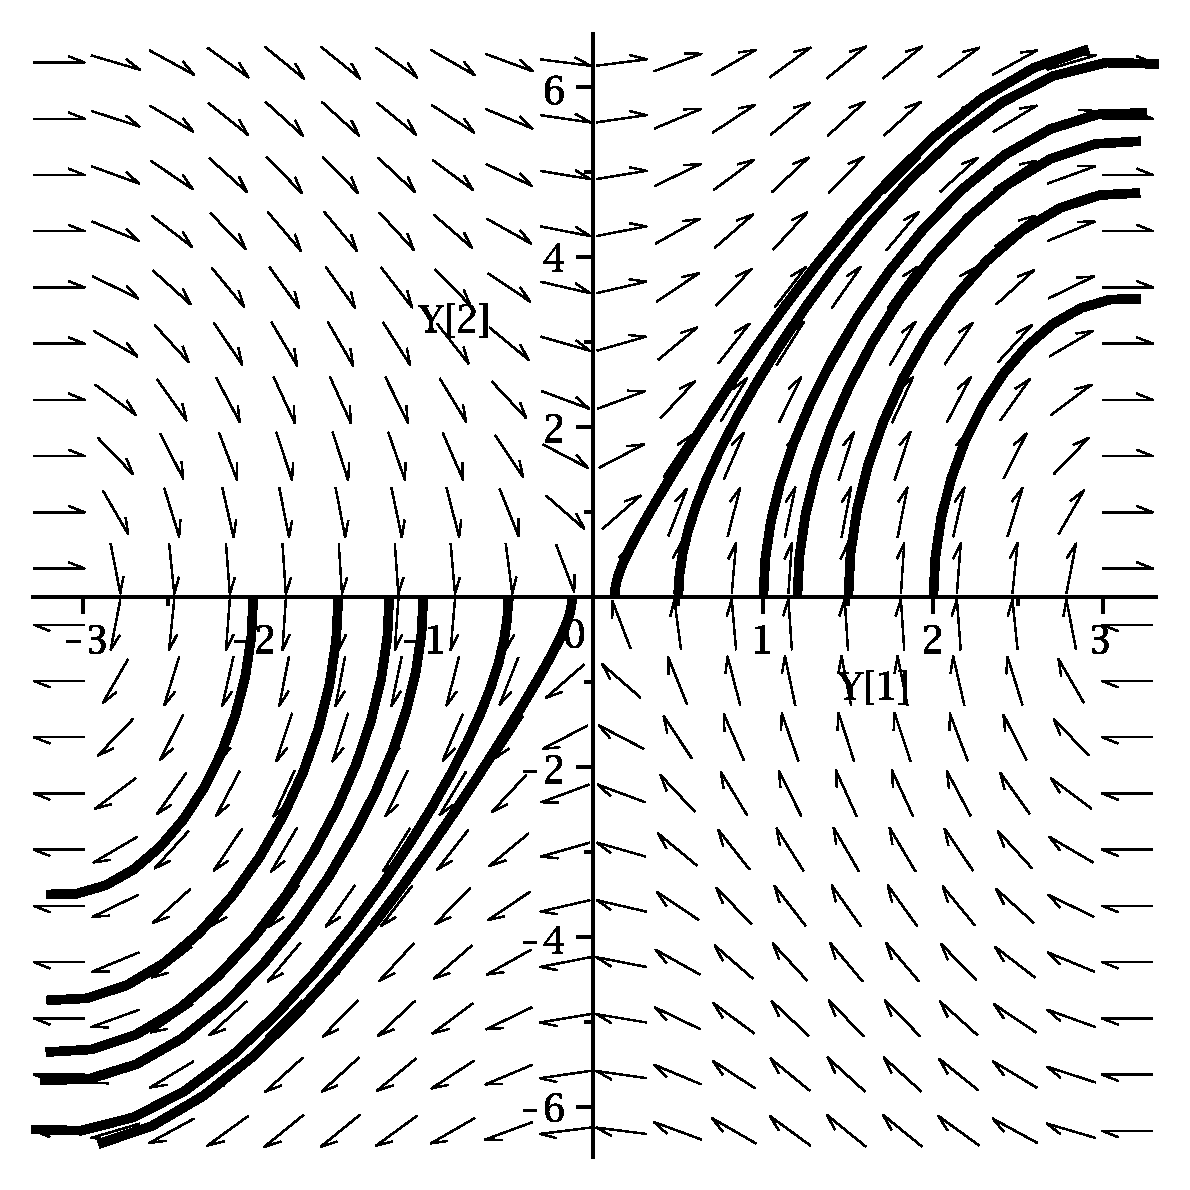
\includegraphics[width=.3\textwidth-0.1]{img/twip_pp_nctrl.eps}\hfill
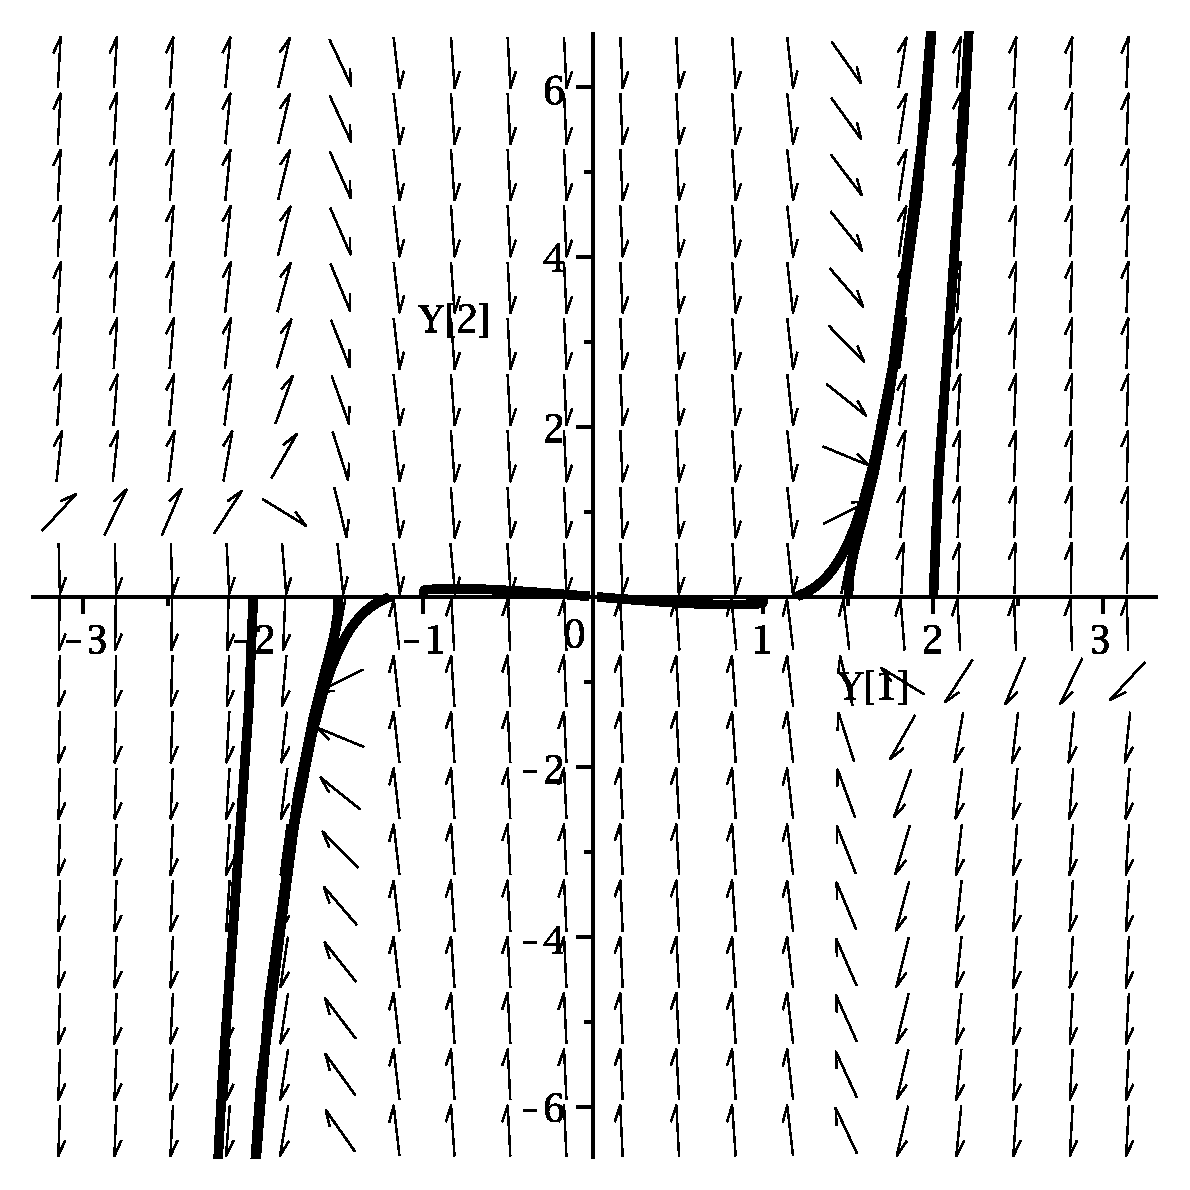
\includegraphics[width=.3\textwidth-0.1]{img/twip_pp_pd_3_10.eps}\hfill
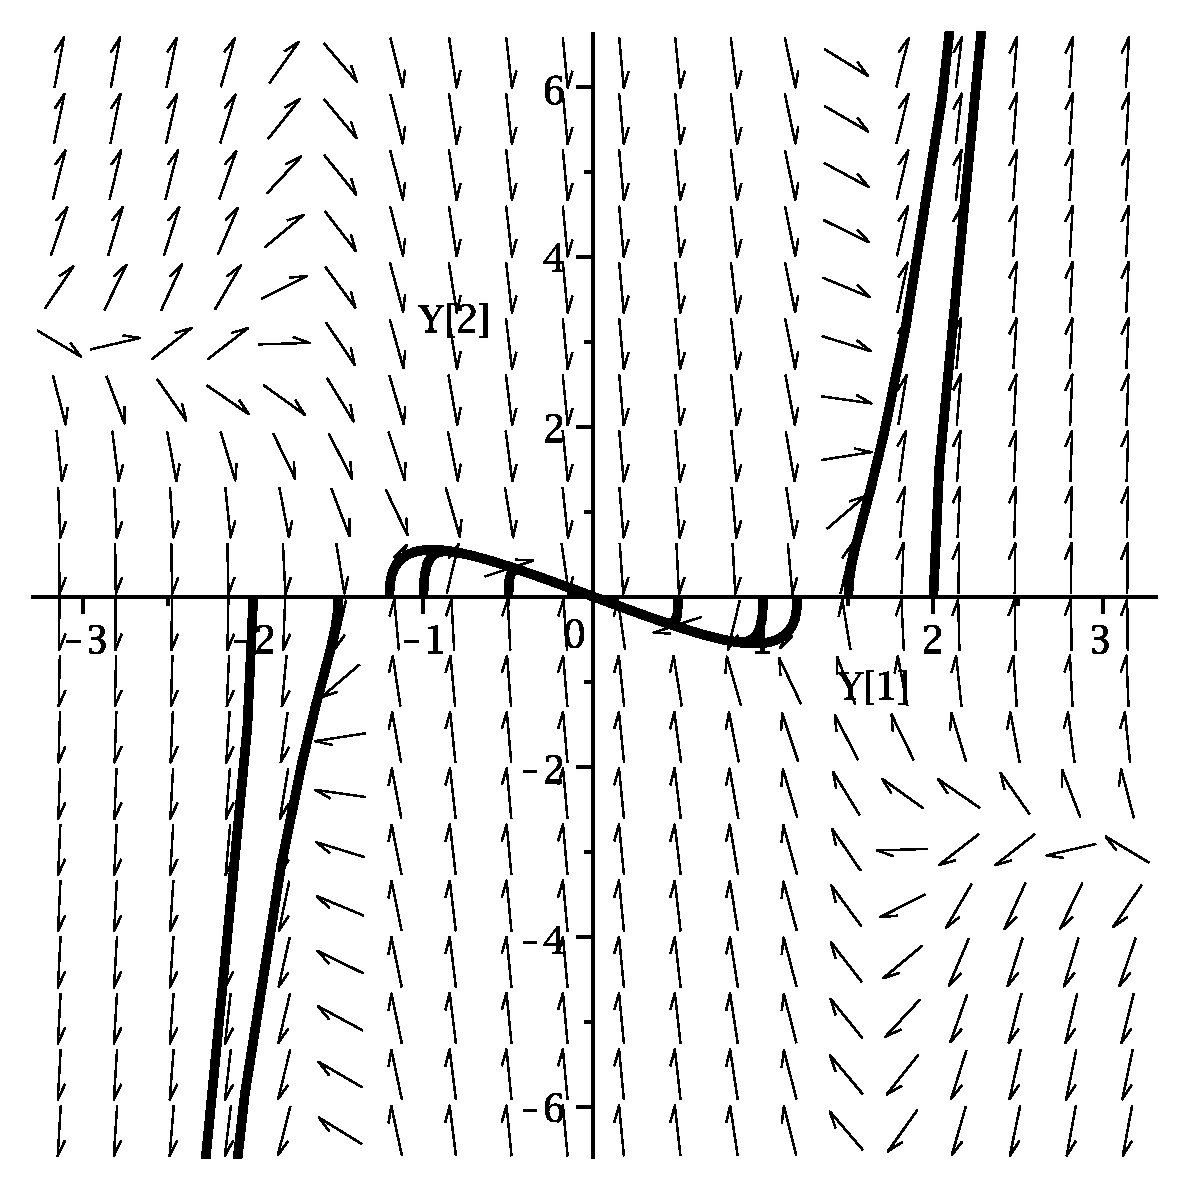
\includegraphics[width=.3\textwidth-0.1]{img/twip_pp_pd_5_5.eps}

\caption{Phase portraits illustrate the benefits of a \gls{pd} controller. On the left, the uncontrolled system acts like any other undamped pendulum system, cycling about the equilibrium point $[y_1,y_2] = [\pi, 0]$. In the middle, a poorly tuned \gls{pd} controller is able to attract system states into an inverted pendulum steady state; the region of attraction is about $y_1 \in [-1.1, 1.1]$.   To the right, new \gls{pd} gains increase this stable region to about $y_1 \in [-1.3, 1.3]$.  }
\label{fig:pdtwippp}
\end{figure}

